\documentclass[12pt]{article}
\usepackage{sbc-template}
\usepackage{graphicx,url}
\usepackage{gensymb}
%\usepackage[brazil]{babel}   
\usepackage[latin1]{inputenc}  
\usepackage{caption3}
\captionsetup{font=footnotesize}

\hyphenation{ algo-ritmos co-lher }
     
\sloppy

\title{PlantGoshi\\ Projeto Integrador III - Sistema Aut\^onomo}

\author{Anderson J. Silva, Felipe R. de Luca, Nelson J. Dressler }


\address{Bacharelado em Ci\^encia da Computa\c c\~ao -- Centro Universit\'ario Senac - Santo Amaro \\
  S\~ao Paulo - SP - Brasil \\ 2015
}
\begin{document} 

\maketitle
     
\begin{resumo} 
O projeto foi desenvolvido para a disciplina Projeto Integrador III: Sistema Aut\^onomo,
com o objetivo de aplicar t\'ecnicas e implementar algoritmos de vis\~ao computacional
em um jogo de tema livre. Para tal, criamos um jogo digital em 2D, desenvolvido em linguagem C,
onde o jogador deve cuidar de uma \'arvore em seu processo de crescimento, com o objetivo
principal de colher os melhores frutos. Para isso, o jogador ter\'a como ferramenta de
intera\c c\~ao uma varinha m\'agica, que permitir\'a aplicar poderes que interajam
com os elementos dentro do jogo, contribuindo com o crescimento da \'arvore e impedindo
que pragas ataquem os frutos. A intera\c c\~ao da varinha com o jogo ser\'a por
interm\'edio do reconhecimento dela nas imagens capturadas pela c\^amera de video
instalada no computador, processadas por algoritmos baseados em levantamento bibliogr\'afico.

\end{resumo}

\section{Introdu\c c\~ao}

 O Projeto desenvolvido para a disciplina Projeto Integrador III: Sistema Aut\^onomo aborda a quest\~ao sobre
 educa\c c\~ao ambiental. O jogador tem tr\^es minutos para cuidar de uma \'arvore, desde seu crescimento
 at\'e o amadurecimento e colhimento dos frutos. Durante a partida, o jogador dever\'a estar sempre atento
 \`a falta de \'agua e pragas que surgir\~ao para comer os frutos.
   
 O desafio do projeto consiste em estudar, desenvolver e implementar algoritmos de vis\~ao computacional 
 para processamento de imagens, com a finalidade de promover a intera\c c\~ao do jogador com o jogo. Essa
 intera\c c\~ao dever\'a ocorrer exclusivamente atrav\'es da c\^amera de video acoplada ao computador. O jogador
 ter\'a \`a sua disposi\c c\~ao uma varinha m\'agica com uma luz de LED na ponta, que ser\'a reconhecida pelos algoritmos
 e seus movimentos traduzidos como coordenadas de posi\c c\~ao X e Y dentro do jogo. Basicamente a varinha tem
 o funcionamento de um mouse.   
  
\section{O jogo}

 Para vencer os desafios, o jogador tem \`a sua disposi\c c\~ao quatro tipos de poderes especiais: Poder de Regar,
 Poder de Remover Pragas, Poder de Colher Frutos e Poder da M\'usica. Cada um desses poderes tem uma fun\c c\~ao
 diferente no jogo e devem ser utilizadas com cautela, pois quando acionado um desses poderes, os restantes ficar\~ao
 indispon\'iveis por alguns segundos. N\~ao \'e poss\'ivel utilizar mais de um poder por vez.
 
 \subsection{Poderes}
 \subsubsection{Poder de Regar} 
 Com Poder de Regar o jogador garante que a \'arvore ir\'a crescer mais e consequentemente ir\'a
 dar mais frutos. \'E necess\'ario estar sempre atento \`a barra de n\'ivel de \'agua. Nunca regue demais a
 \'arvore e tamb\'em n\~ao a deixe sem \'agua.
 
	\begin{figure}[ht!]
	\begin{center}
		
\includegraphics[scale=1.15]{img/icone_gota.png}
		\footnotesize \caption{Poder de Regar }
	\end{center}
	\end{figure}	
  
 \subsubsection{Poder de Remover Pragas}
 O Poder de Remover Pragas auxilia o jogador a retirar bichos que nascem, evitando assim
 que os frutos sejam comidos. O jogador tem um tempo curto para remover essas pragas, antes que
 elas danifiquem os frutos e a \'arvore.

	\begin{figure}[ht!]
	\begin{center}
		
\includegraphics[scale=1.15]{img/icone_luva.png}
		\footnotesize \caption{Poder de Remover Pragas }
	\end{center}
	\end{figure}	
 
 \subsubsection{Poder da M\'usica}
 O poder da m\'usica auxilia no amadurecimento mais r\'apido dos frutos. O jogador aplica diretamente esse poder em cima
 do fruto que deseja.
 
	\begin{figure}[ht!]
	\begin{center}
		
\includegraphics[scale=1.15]{img/icone_nota_musical.png}
		\footnotesize \caption{Poder da M\'usica}
	\end{center}
	\end{figure}	

 \subsubsection{Poder de Colher}
 A pontua\c c\~ao final da partida do jogo est\'a diretamente ligada ao Poder de Colher. Existe um momento ideal para colher o
 fruto, que \'e quando ele est\'a vermelho e saud\'avel. Caso seja colhido antes da hora ou depois, o jogador perder\'a
 pontos. Muita aten\c c\~ao caso o fruto esteja com praga. Se isso ocorrer, ser\'a necess\'ario remov\^e-la antes de
 colher o fruto.
 
	\begin{figure}[ht!]
	\begin{center}
		
\includegraphics[scale=1.15]{img/icone_cesta.png}
		\footnotesize \caption{Poder de Colher}
	\end{center}
	\end{figure}	

 \subsection{Varinha m\'agica}
 Com a varinha m\'agica o jogador poder\'a interagir com os elementos dentro do jogo como sele\c c\~ao de poderes, regar e remo\c c\~ao
 de pragas. Ao selecionar um poder a luz na ponta da varinha ir\'a assumir a cor desse poder, indicando que ele foi selecionado e est\'a ativo.
 Se n\~ao houver luz, significa que a sele\c c\~ao de poderes est\'a desabilitada temporariamente. Caso a luz seja a cor branco, ent\~ao
 est\'a dispon\'ivel selecionar qualquer poder.
 
 Para interagir com o jogo, basta mover a varinha em frente \'a tela do computador e um cursor na tela ir\'a indicar qual a posi\c c\~ao
 atual da varinha dentro do jogo. Para selecionar o poder desejado, \'e necess\'ario posicionar o cursor por dois segundos em cima desse poder.
 O poder foi selecionado quando a luz na ponta da varinha mudar de cor. 

	\begin{figure}[ht!]
	\begin{center}
		
\includegraphics[scale=0.5]{img/varinha.png}
		\footnotesize \caption{Varinha m\'agica com LED na ponta.}
	\end{center}
	\end{figure}	

\subsection{Layout}

	\begin{figure}[ht!]
	\begin{center}
		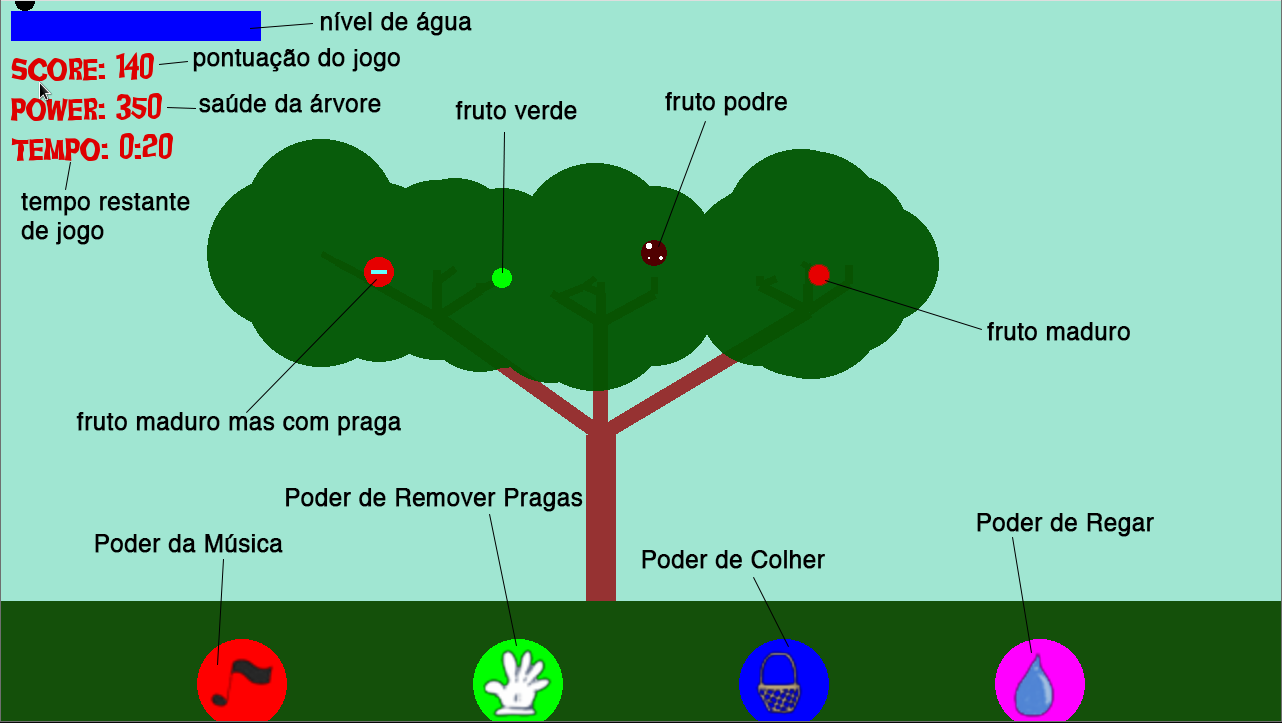
\includegraphics[scale=0.3]{img/tela_jogo.png}
		\footnotesize \caption{Primeira vers\~ao da tela do jogo. Os gr\'aficos ser\~ao alterados para a vers\~ao final do jogo.}
	\end{center}
	\end{figure}	

\subsection{Etapas}
A partida do jogo \'e dividida em tr\^es principais etapas: 

\begin{enumerate}
\item \textbf{Nascimento e Crescimento da \'Arvore:} o jogador dever\'a estar atento a regar a \'arvore sempre que
necess\'ario e, ao mesmo tempo, combater ervas daninhas que ir\~ao crescer ao p\'e dela.
\item \textbf{Amadurecimento dos Frutos:} os frutos ir\~ao crescer mais r\'apido se o jogador utilizar notas musicais.
Tamb\'em ir\~ao crescer pragas nesses frutos, que podem ser combatidas com o poder de remo\c c\~ao de pragas.
\item \textbf{Colhimento dos Frutos:} \'e o momento no qual os frutos cresceram e amadureceram
 o suficiente para serem colhidos, contabilizando pontos para o jogador.
\end{enumerate}

\section{Vis\~ao Computacional}

Compreendendo a parte de vis\~ao computacional, foi realizado um levantamento bibliogr\'afico
referente ao processamento digital de imagens, reconhecimento de padr\~oes em imagens, opera\c c\~oes
aritm\'eticas e um estudo aprofundado sobre os modelos de cores, sua natureza e suas caracter\'isticas principais.

\subsection{Algoritmos utilizados\label{sec:alg}}
\subsubsection{HSV e RGB}
Cada pixel de uma imagem extra\'ida da c\^amera do computador no modelo de cores RGB (Red, Green, Blue) \'e convertido em
HSV / HSB (Hue, Saturation, Value / Brightness), permitindo descobrir o grau da cor pura (Matiz), as faixas representada por cada cor,
a porcentagem de satura\c c\~ao da cor (Pureza) e a porcentagem de brilho (Valor).

O H \'e a matiz e \'e medida em graus compreendendo valores de 0\degree a 359\degree.
A faixa de cada uma das seis cores principais (prim\'arias e secund\'arias) \'e definida numa margem de 60 graus.
As faixas s\~ao classificadas da seguinte maneira: Vermelho (0\degree a 59\degree), Amarelo (60\degree a 119\degree), Verde (120\degree a 179\degree),
Ciano (180\degree a 239\degree), Azul (240\degree a 299\degree) e Magenta (300\degree a 359\degree).
O S \'e a satura\c c\~ao e \'e medida em porcentagem nos valores de 0 a 100\%.
Finalmente, o V \'e o brilho e medido tamb\'em em porcentagem, (0 a 100\%). Como observa\c c\~ao importante, \'e possível notar
que as cores branco e preto s\~ao definidas de acordo com o valor de V: quando se aproxima de 0, emite a cor preta,
e quando se aproxima de 100, branca.

Por exemplo, para reconhecer a luz do LED, \'e poss\'ivel por interm\'edio de uma porcentagem alta
do V (Valor de brilho) e sua cor pela faixa de H (Matiz).

Para manipular essa representa\c c\~ao, foi necess\'ario a cria\c c\~ao de uma estrutura chamada Pixel
que deve armazenar todos os dados de cores de apenas um pixel e a implementa\c c\~ao de dois algoritmos
que compreendem as convers\~oes nos dois sentidos: RGB para HSV e HSV para RGB.

A fim de padronizar, foram implementadas tamb\'em algumas fun\c c\~oes de formata\c c\~ao: convers\~ao de
um valor decimal para porcentagem (S e V), convers\~ao de um grau para um valor de 0 a 5 (H) e convers\~ao
de canais de cores RGB em um valor decimal entre 0 e 1.

Al\'em disso, foram desenvolvidas fun\c c\~oes complementares de m\'aximo e m\'inimo dentre tr\^es valores (R, G e B).

	\begin{figure}[ht!]
	\begin{center}
		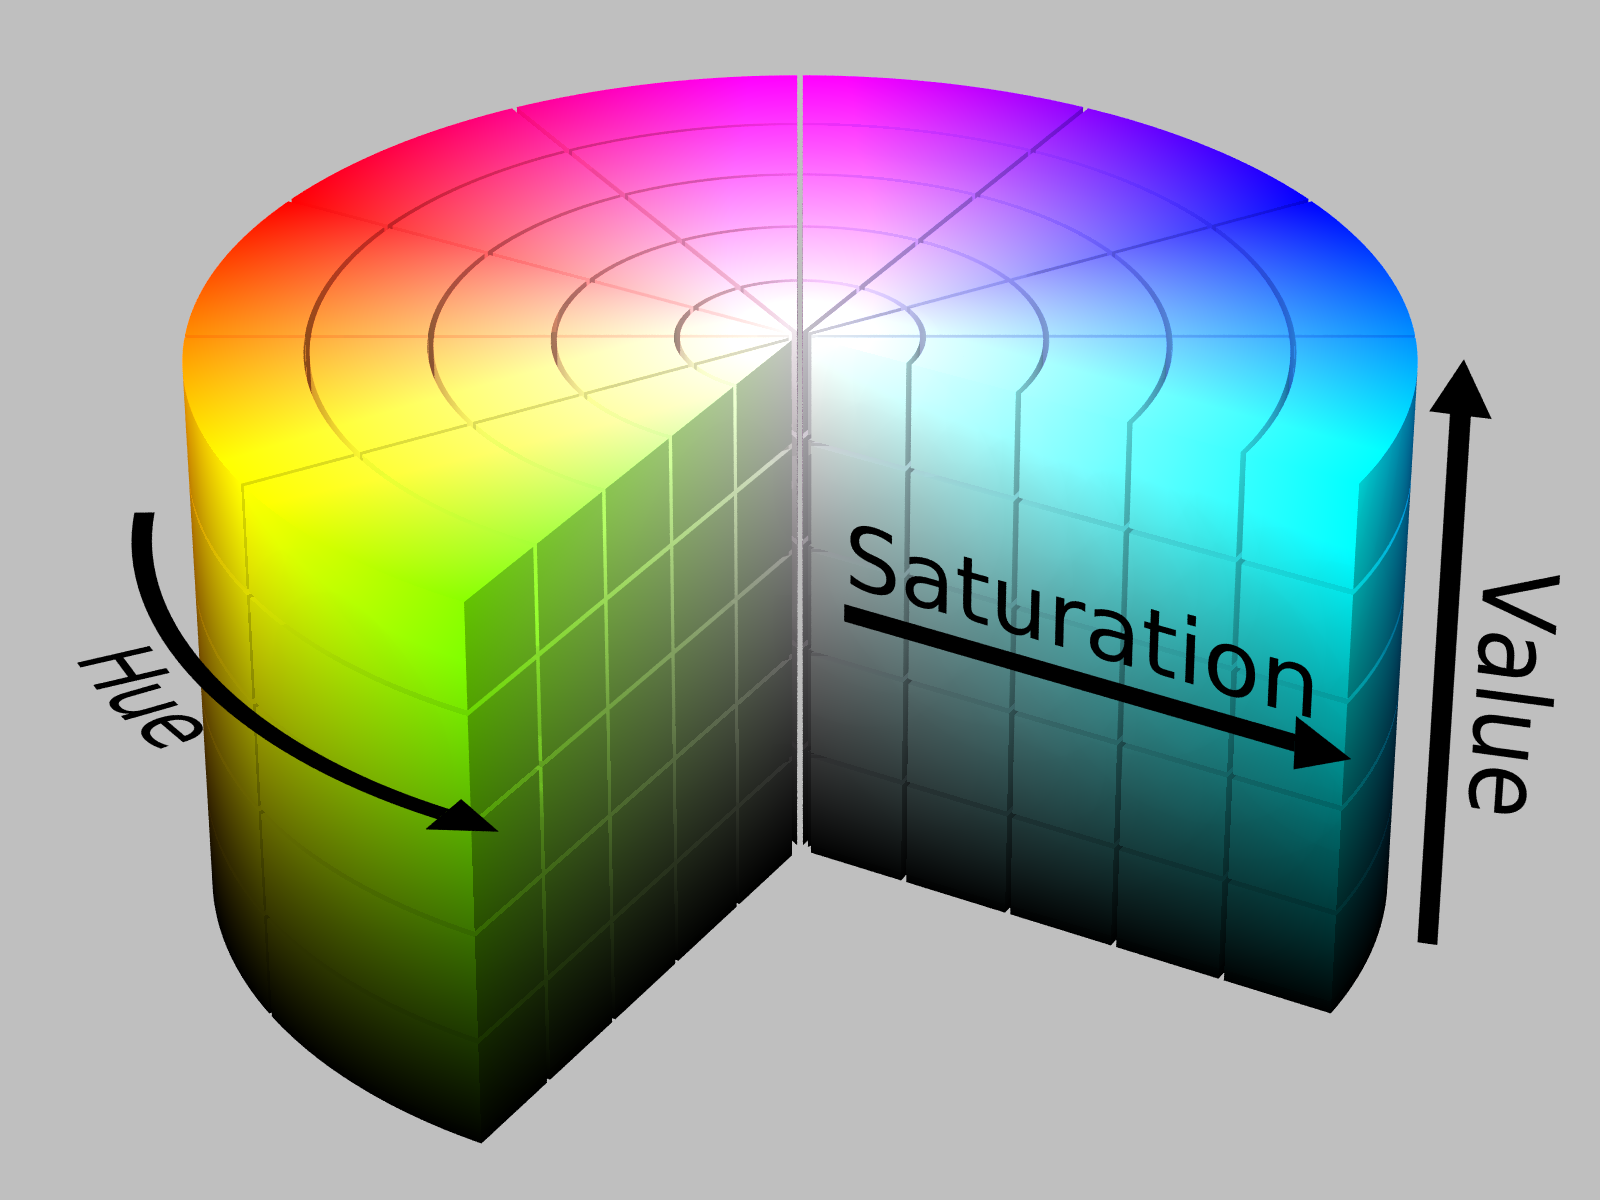
\includegraphics[scale=0.15]{img/HSV_color_solid_cylinder_alpha_lowgamma.png}
		\footnotesize \caption{Representa\c c\~ao tridimensional do espa\c co de cor HSV. Cr\'editos: SharkD. http://en.wikipedia.org/wiki/HSL\_and\_HSV }
	\end{center}
	\end{figure}	

\subsubsection{Escala de cinza}
Os valores RGB de um pixel podem ser convertidos em escala de cinza por uma s\'erie de m\'etodos.
Com esse fim, foi escolhido o m\'etodo de escalas fixas correspondendo a cada um dos canais RGB.
\'E efetuada a seguinte opera\c c\~ao sobre cada pixel:

\texttt{\small \textbf{R} x 0,3 + \textbf{G} x 0,51 + \textbf{B} x 0,18}

\noindent Dessa maneira, cada pixel assume apenas um valor e, ao mesmo tempo, \'e mantida uma escala para cada valor RGB,
levando em considera\c c\~ao a sua maior tonalidade.

	\begin{figure}[ht!]
	\begin{center}
		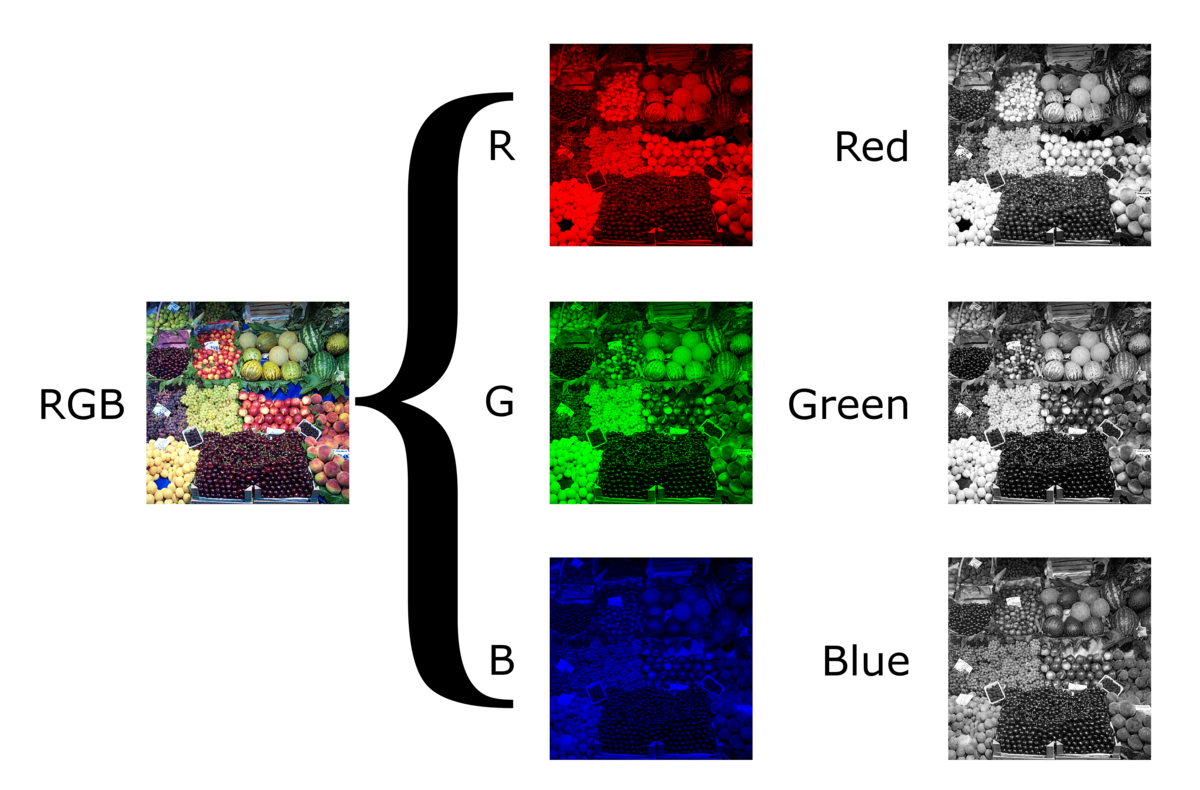
\includegraphics[scale=0.8]{img/1200px-Beyoglu_4671_tricolor.png}
		\footnotesize \caption{Convers\~ao de canais de cores para escala de cinza. Cr\'editos: Nevit Dilmen. http://en.wikipedia.org/wiki/Grayscale }
	\end{center}
	\end{figure}	

\subsubsection{Redu\c c\~ao de cores}
A redu\c c\~ao de cores \'e uma t\'ecnica que tem por objetivo facilitar o reconhecimento de uma regi\~ao espec\'ifica,
diminuindo as cores vis\'iveis e tornando uma regi\~ao mais destacada e isolada que as demais.
Para tal, \'e usada a seguinte opera\c c\~ao sobre cada canal RGB:

\texttt{\small Canal = Canal x Fator + Fator / 2}

\noindent sendo o fator um valor inteiro que define a propor\c c\~ao da quantidade cores que se quer diminuir na imagem.
Exemplos de Fatores: 2, 16, 64, 128. Quanto maior o fator, menor a quantidade de cores vis\'iveis.

	\begin{figure}[ht!]
	\begin{center}
		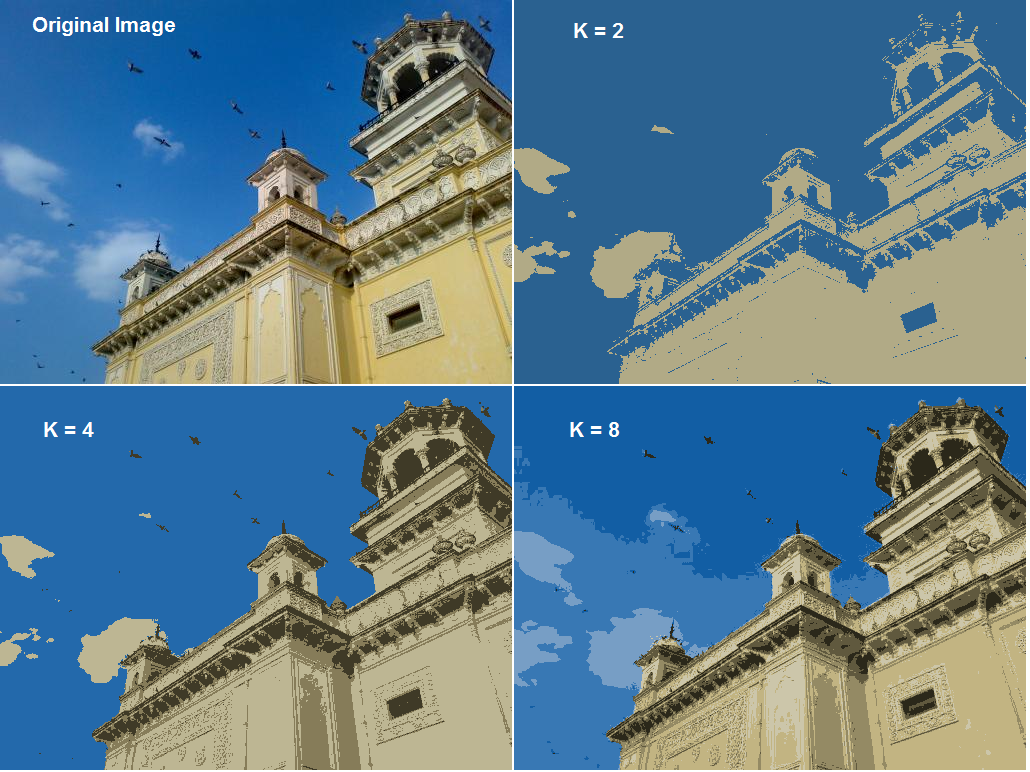
\includegraphics[scale=0.3]{img/kmeansout.png}
		\footnotesize \caption{Redu\c c\~ao da quantidade de cores de acordo com valor do par\^ametro K. Fonte: http://opencvpython.blogspot.com.br/2013/01/k-means-clustering-3-working-with-opencv.html }
	\end{center}
	\end{figure}	

\subsubsection{Controle de massas}
Visando uma defini\c c\~ao exata e correta do ponto central que deve ser devolvido pela fun\c c\~ao da vis\~ao computacional,
foi necess\'ario a implementa\c c\~ao de um mecanismo para ter ideia caso outras massas brancas al\'em da principal (o LED)
est\'a sendo retornada e, com isso, comprometendo a jogabilidade do jogo.

Essa fun\c c\~ao analisa a vizinhan\c ca de cada um dos pixels da imagem contabilizando as massas brancas presentes em tela.

Para isso, \'e criada uma estrutura bidimensional chamada Matriz de V\'ertices, onde cada v\'ertice armazena informa\c c\~oes
relevantes sobre cada pixel: valor definindo se o pixel está aceso (1 - branco) ou apagado (0 - preto) e o numero de massa
definido por uma vari\'avel contadora.

Ao final, o algoritmo retorna um n\'umero inteiro compreendendo a quantidade de massas brancas encontradas.

\subsubsection{Eros\~ao e dilata\c c\~ao}
A Eros\~ao e a Dilata\c c\~ao s\~ao t\'ecnicas de filtragem com o objetivo de reduzir ru\'idos presentes na imagem,
que possam dificultar a detec\c c\~ao de pontos principais na tela.

Os ru\'idos podem ser causados por uma s\'erie de fatores, dentre eles limita\c c\~oes da c\^amera presente no computador
e presen\c ca de pontos isolados na tela que tenham caracter\'isticas similares aos procurados.

A Eros\~ao trata de eliminar os pontos isolados na imagem, os quais n\~ao possuem outros em destaque em sua vizinhan\c ca.

A Dilata\c c\~ao trata de aumentar os pontos isolados na imagem, consistindo no processo contr\'ario da Eros\~ao.

Com uma sequ\^encia razo\'avel de opera\c c\~oes de Eros\~ao e Dilata\c c\~ao, a quantidade de ru\'idos \'e descartada,
ao mesmo passo que a regi\~ao que deve ser destacada \'e mantida em seu tamanho original.

	\begin{figure}[ht!]
	\begin{center}
		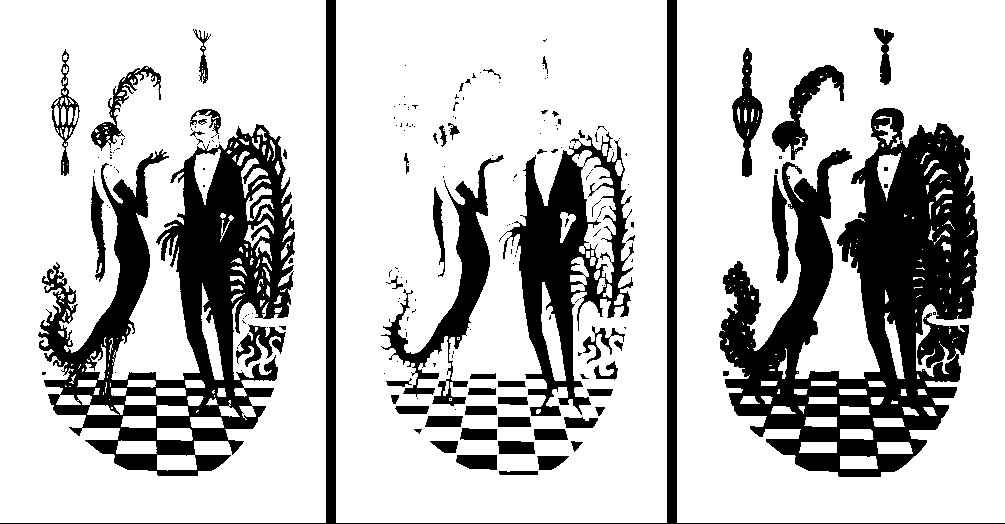
\includegraphics[scale=0.3]{img/erodeDilate.png}
		\footnotesize \caption{Esquerda: Imagem original. Meio: eros\~ao. Direita: dilata\c c\~ao. Fonte: http://visiblevisible.org/teaching/setpixel/students/katherine/images/erodeDilate.png }
	\end{center}
	\end{figure}	
	
\subsection{Aplica\c c\~ao dos algoritmos}
Utilizando os algoritmos descritos em \textbf{~\ref{sec:alg}}, foi criada uma fun\c c\~ao de vis\~ao computacional que aplica cada um desses
algoritmos para retirar informa\c c\~oes sobre os pixels da imagem.

Primeiro, o canal RGB \'e convertido em HSV antes e ap\'os a aplica\c c\~ao do efeito de redu\c c~ao de cor para
cruzar as informa\c c\~oes de luminosidade com a cor espec\'ifica do LED a ser detectado pelo algoritmo, respectivamente.

Ap\'os isso feito, \'e armazenado numa Matriz Bin\'aria a regi\~ao do LED, definindo o valor 1 para pixel com
a cor e luminosidade detectada e 0 para n\~ao detectada.

Essa matriz passa por uma sequ\^encia de Eros\~oes e Dilata\c c\~oes at\'e que a regi\~ao principal seja destacada
e os ru\'idos eliminados. Essas opera\c c\~oes ocorrem por interm\'edio de uma matriz chamada de M\'ascara.

Posteriormente, na matriz bin\'aria \'e verificada a quantidade de massas brancas presentes e, caso haja mais de uma,
o LED \'e simplesmente ignorado.

Caso haja apenas uma massa, \'e calculada a m\'edia das posi\c c\~oes x e y onde os pixels est\~ao acesos e \'e devolvida
uma coordenada (x, y) central. Para isso, \'e foi criada uma estrutura chamada Vis\~ao Computacional que armazena
o par ordenado da regi\~ao central do LED, a cor detectada pelo mesmo e faixa de luminosidade que \'e testada no momento
da calibra\c c\~ao da c\^amera pelo algoritmo.

\section{Simula\c c\~ao da \'arvore}

Adotamos a estrutura de dados de \'arvore tern\'aria para construir a \'arvore do jogo. Essa estrutura \'e basicamente constituida
em pontos de crescimento que se dividem no m\'aximo em tr\^es partes cada um. Essas partes d\~ao origem aos galhos que crescem at\'e
determinado tamanho, decidido aleat\'oriamente. As pontas de cada galho s\~ao novos pontos de crescimento,
que se dividem de novo e d\~ao origem a novos galhos

Para que simula\c c\~ao tenha um aspecto e comportamento mais pr\'oximo de uma \'arvore, elaboramos uma solu\c c\~ao que inclui
a mat\'eria estudada na disciplina de Estrutura de Dados e elaboramos algoritmos para simular o crescimento da \'arvore,
dos galhos e dos frutos. Basicamente a \'arvore cresce de acordo com um valor de energia de crescimento fornecida
a ela logo no in\'icio do jogo. Uma parte dessa energia \'e consumida pelo tronco e o restante \'e distribuido
de maneira aleat\'oria para os pr\'oximos galhos que ir\~ao nascer, de acordo com o seguinte crit\'erio: \\

 \texttt{\footnotesize{\textbf{SE} galho.energiaConsumida == ((galho.energiaLimite * 50) / 100) \textbf{E} galho.temFilhos == FALSO 
        \textbf{ENT\~AO} galho.criarFilhos = SIM}} \\


Isso se repete at\'e que n\~ao haja mais energia suficiente
para repassar ao galho seguinte. O jogador tem a oportunidade de fornecer mais energia ao longo da partida, o que
ir\'a proporcionar uma \'arvore mais desenvolvida e com mais frutos para serem colhidos.

	\begin{figure}[ht!]
	\begin{center}
		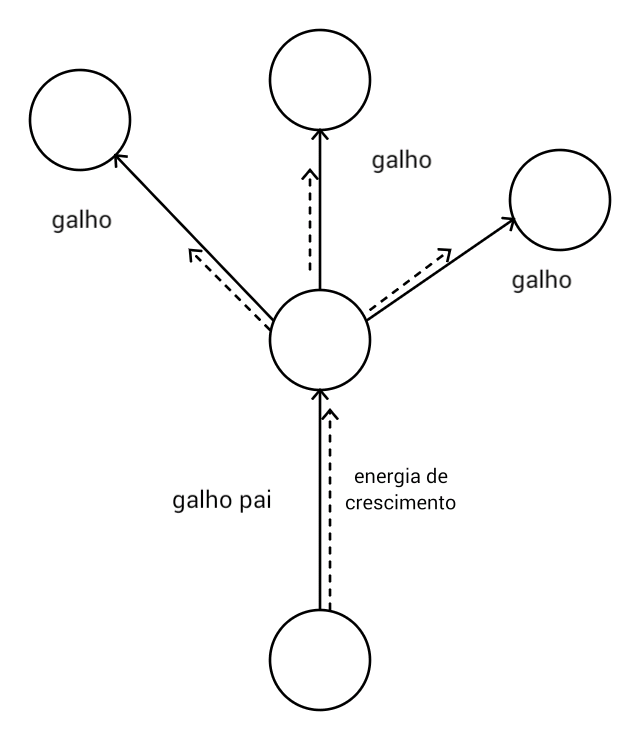
\includegraphics[scale=0.2]{img/PI3_Ponto_Crescimento.png}
		\caption{\footnotesize {Crescimento dos galhos e energia transferida de pai para filho.} }
	\end{center}
	\end{figure}	
	
\subsubsection{Crescimento}
Para que os galhos crescam controladamente mas mantendo certa diferencia\c c\~ao em tamanho e
dire\c c\~ao entre um e outro, estabelecemos um crit\'erio que chamamos de energia de crescimento e energia limite.
A energia limite determina o quanto cada  galho da \'arvore vai crescer e \'e estabelecido atrav\'es de uma porcentagem,
calculada a partir do total de energia de crescimento fornecida para o galho, o n\'ivel de altura desse galho e a energia
limite da \'arvore:

  \texttt{\footnotesize{galho.energiaLimite = (energiaRecebida * (arvore.energiaLimite - (galho.profundidade * 2)) / 100)}}

O valor da energia limite pode
ser alterado de acordo com a intera\c c\~ao do usu\'ario ao longo do jogo, o que pode proporcionar uma \'arvore mais
mais ou menos desenvolvida.

Enquanto os galhos crescem eles podem dar origem a novos galhos. Isso \'e determinado ap\'os ser consumida uma determinada
quantidade de energia de crescimento fornecida ao galho, o que permite que a simula\c c\~ao de crescimento da \'arvore
fique mais natural. A \'unica exce\c c\~ao \'e o tronco da \'arvore, que tem o crescimento
mais controlado:

\texttt{\footnotesize{\textbf{SE} galho.energiaConsumida < galho.energiaLimite \textbf{E} galho.energiaRecebida > 0
\textbf{ENT\~AO} galho.crescer}}

\subsubsection{Pontos de crescimento de frutos e folhas}
Os pontos de crescimento de frutos e folhas s\~ao determinados de acordo com o m\'inimo de energia que o galho
tem para crescer. Caso esse valor seja igual ou abaixo de determinado crit\'erio, o algoritmo de simula\c c\~ao assume
que n\~ao ir\~ao surgir novos galhos a partir do galho atual, ainda durante a fase de crescimento. Com isso determinado,
o galho passa a produzir folhas e frutos ao inv\'es de novas ramifica\c c\~ao de galhos.

	\begin{figure}[ht!]
	\begin{center}
		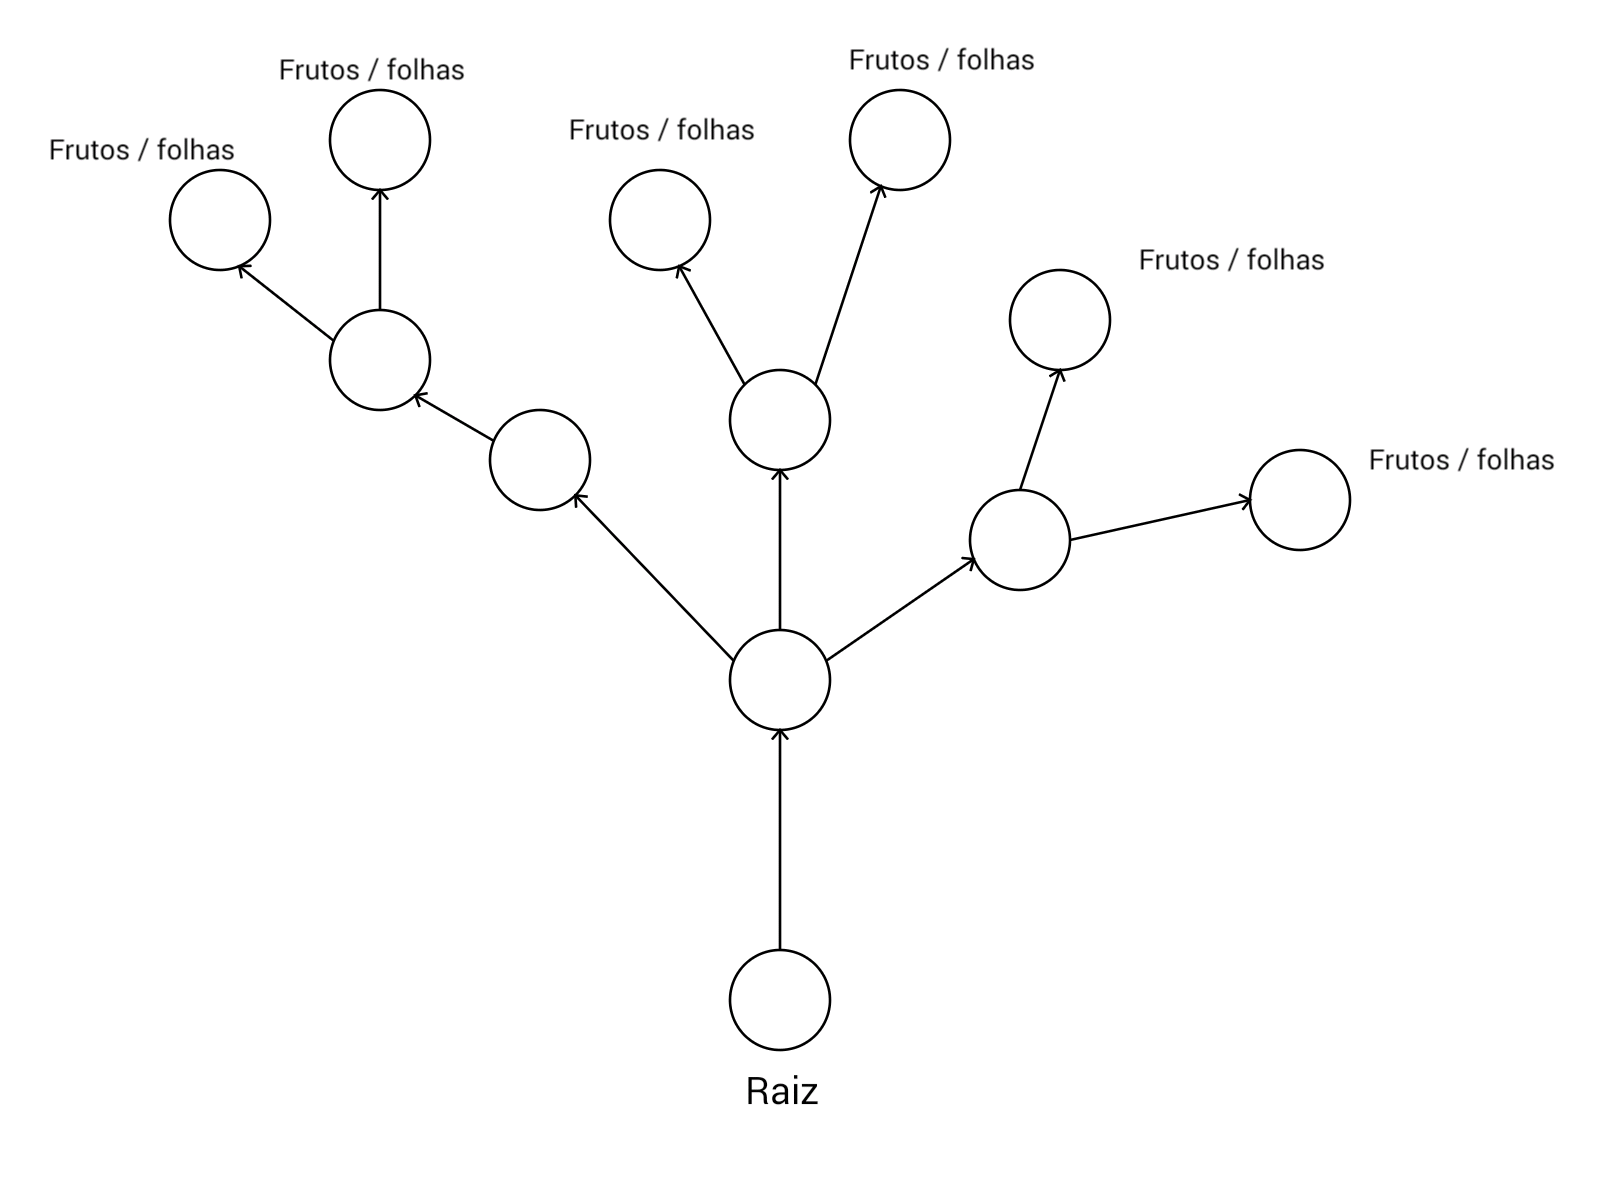
\includegraphics[scale=0.15]{img/PI3_Arvore.png}
		\footnotesize \caption{Estrutura da \'arvore e pontos de crescimento de frutos e folhas }
	\end{center}
	\end{figure}	

\subsection{Primeiros experimentos}
Para o reconhecimento de uma cor emitida por um LED do Arduino, fizemos uma otimiza\c c\~ao f\'isica
com um peda\c co de papel que reduzisse o brilho da luz, por\'em ainda n\~ao \'e suficiente para
o reconhecimento total.

Como experimentos necess\'arios, temos o reconhecimento da luminosidade para verificar
a proximidade da luz com a c\^amera e uma otimiza\c c\~ao afim de isolar a cor do LED,
ignorando as outras cores similares e aparentes na c\^amera.

\section{Bibliotecas}
\subsection{OpenCV 2.4.11}
OpenCV (Open Source Computer Vision Library)
\'e uma biblioteca de c\'odigo aberto de vis\~ao computacional e aprendizado de m\'aquina,
desenvolvida para dar suporte a aplicativos que requerem processamento de imagens.
  
\subsection{Allegro 5.0}
O Allegro \'e uma biblioteca multiplataforma de programa\c c\~ao voltada para desenvolvimento de jogos. Ela
oferece suporte para programa\c c\~ao baixo n\'ivel em C e C++, ou seja, fornece ferramentas para que o usu\'ario
desenvolva sua pr\'opria programa\c c\~ao de jogo.
\subsection{Arduino-Serial}
Biblioteca de c\'odigo aberto em linguagem de programa\c c\~ao C, que oferece suporte a
comunica\c c\~ao via porta serial do computador com o Arduino.

\subsection{Linguagens de programa\c c\~ao}
O projeto inteiro foi desenvolvido em linguagem C padr\~ao c99.

\section{Equipamentos}
\begin{itemize}
\item C\^amera de captura de v\'ideo
\item Placa controladora Arduino Uno
\item LED RGB
\item Computador (desktop ou notebook)
\end{itemize}

\nocite{*}

\section{Bibliografia}
\bibliographystyle{sbc}
\bibliography{plantgoshi}


\end{document}
